\section{R-CNN}
% {
%     \color{red}
%     \noindent TODO: \\
%     - learn caffe for feature extraction \\
%     - learn Support Vector Machines(SVM) for classifying from feature vector
% }

R-CNN, also known as regional-based convolutional neural networks, is an object detection algorithm. The algorithm was developed by a group of researchers at UC Berkeley in 2015. Since its development, the R-CNN model has revolutionized the field of computer vision. The model was designed to detect up to 80 different types of objects in images and provide large-scale object recognition capabilities. Additionally, before the existence of RCNN, most algorithms in object recognition task used support vector machine (SVM) with blockwise orientation histograms like Histogram of Oriented Gradients (HOG) or Scale-Invariant Feature Transform (SIFT). SVM dominated the space until 2012. In 2012, a CNN algorithm showed an astounding image classification accuracy on ImageNet Large Scale Visual Recognition Challenge (ILSVRC). Since then, more studies have been created into developing and improving algorithms utilizing CNN. The R-CNN model is our first attempt to build an object detection model that extracts features using a pre-trained CNN.

In a board picture, R-CNN model is composed of three modules. The first module's purpose is to generate regions of interest (ROI) i.e., regions that possibly contain an object. The second module utilizes a CNN to extract out feature vector from each proposed region. The third module then performs classification for each region using a pre-trained SVM algorithm on the feature vectors provided by the second module. As we can see R-CNN algorithm tries to find the location of each object, extract the object features, and classify these features. Next, we will dive deeper into each module of R-CNN.

\subsection{The First Module: Region Proposal}
In the first module, the algorithm used in this step must be able to propose some region of interest (ROI). A region of interest is a smaller part of the original image that could contain an object.

Given this problem, one might consider the bruce-force method by examining every small rectangle area of the original image as a potential region of interest in a systematic way. This method is the main concept behind the sliding-window technique, a type of exhaustive search algorithm used in the region proposal task. The sliding window technique involves running a window of a predefined size across the image, such that each subsection of the image is considered as a potential region proposal. Like the CNN kernel, the windows' size, stride, and padding are all customizable and can be adjusted to suit different types of images. In addition, multiple scales can also be incorporated into the sliding window technique, which allows for more robust performance in scenarios where objects may appear at different sizes within the same image. Since the sliding window technique examines every location within the image by considering every pixel as part of some ROI, it will not miss any potential object location. However, considering every location in the image as a ROI is unnecessary due to objects most likely not appearing everywhere in the image. Furthermore, classifying every sub-image at different sizes will require tremendous computational power. Therefore, even though it allows our model to detect all possible locations, the sliding window technique should not be used in autonomous cars' vision because it is computationally expensive.

{\color{red} consider describe segmentation statregy: segmentation able to generate multiple foreground and background segmentation and is trained to scoring if a forground segment is an object}

In recent years, many study have show interest in improve the efficient of region proposal algorithm. One notable algorithm that given the same strength as the sliding window technique is selective search. Selective search was designed to combines the strength of both exhaustive search and segmentation \cite{uijlings_selective_search_2013}. The strength that selective search inherits from sliding windows is the ability to find all the possible locations that can be a potential region of interest. Additionally, selective search ustilize the underlying image structure to cluster pixels into different regions, taken from the strength of segmentation technique. Selective search also aim to complete three goals. These three goals are capture all scale, diversification, and fast to compute. Capture all scale is the idea that the algorithm must be able to detect object at different size in the image. Next, diversification requirement refer to method of grouping region. The algorithm must be able to combine region contain part of an object into one region. Additionally, for instance like a person inside a car or person in front of a car, the algorithm must be able to seperate the region for the car and the region for the person under diversification requirement. Lastly, fast to compute require the algorithm to not demain heavy computational power.

As for selective search overall behavior. It can be thought as two steps. The first step is perform bottom-up segmentation -- descibed in Efficient Graph-Based Image Segmentation by Felzenszwalb and Huttenlocher \cite{felzenszwalb_huttenlocher_2004} -- to generate initial sub-segmentation. The second step is combine similar sub-segmentation recursive using a similarity score between subsegment. The similarity score is a combination of four similarity grouping criteria. These four criteria are color similarity, texture similarity, size similarity, and fill similarity \cite{uijlings_selective_search_2013}. The reason that color and texture similarity between regions is needed is due to same object mostlily will have the same texture or shade of color. In the original paper, the color and texture similarity criteria score can be descibed by an equation only based on fixed number of values taken from histogram of each color channel. Thus, these two similarity score require minimal to no computational power to compute. Similarly, two region that have majority of the area overlap on each other are most likely described the same object. Therefore, the use of fill similarity score allow the algorithm to merge regions that are mostly overlap and keep regions that are not overlaping seperate from each other. The fill similarity score can be caculated using the following equation: 
%
\begin{equation*}
    S_{fill}(r_i, r_j) = 1-\frac{size(BB_{ij})-size(r_i)-size(r_j)}{size(image)}
\end{equation*}
%
where $r_i, r_j$ are two considering ROI, and $BB_{ij}$ is the bounding box around $i$ and $j$. Lastly, the similarity in size between two regions take into consideration to make sure ensures that the algorithm identify all locations for different object at different scale. The size similarity score can be caculated using the following equation: 
%
\begin{equation*}
    S_{size}(r_i, r_j) = 1-\frac{size(r_i)+size(r_j)}{size(image)}
\end{equation*}
%
where $r_i, r_j$ are two considering ROI. As we can see, the similarity score computation is fast and take into accout the diversify of the image data set. With this two steps, selective search can quickly classify foreground and background, then downsampling number of potential ROI existed in forground segmentation. Therefore, by utilize selective search allow the model to reduce number of falsify ROI compare to sliding window and require lower computational power.

In the original paper of R-CNN, in the first module -- region proposal -- utilize selective search algorithm \cite{Girshick_R_CNN_2013}. However, as mention before, the R-CNN model can be thought of as three seperate modules, thus one can experiment R-CNN with different region proposal technique.

\subsection{The Second Module: Feature Extraction With CNN}
One the first module of R-CNN finish generated all regions of interest within an image, it give these generated ROI to the AlexNet architect for feature extraction \cite{Girshick_R_CNN_2013}. AlexNet, a CNN architect, was proposed by Alex Krizhevsky under the advising of Ilya Sutskever and Geoffrey E. Hinton at university of Toronto in 2012 \cite{AlexNet_2017}. AlexNet was trained on the ImageNet, which is the largest images data set at the time. As AlexNet requrie it input to have a fix resolution with same width and height, the images in ImageNet was down-sampled to fixed size of $256 \times 256$. Prior to publish, AlexNet enter ILSVRC-2010 competition and achieves top-1 error rates of 37.5\%. In other words, the model give the highest score to the correct label 37.5\% of the times. In the same copetition, AlexNet also achieve top-5 error rates of 17.0\%, i.e, the correct label is in the top 5 predicts 17\% of the times. 

% \subsubsection{AlexNet}
AlexNet is considered as one of the major break through in the use of CNN. As of 2012, AlexNet is one of the largest neural network ever proposed, with 60 million parameters and 650,000 neurons. AlexNet's architecture consist of eight learned layers. There are five convolutional layers, followed by three fully connected layers. However, due to hardware limmitation at the time, a large network like AlexNet is not possible to fit in one GPU. For that reason, the model's architecture is spreaded into two different GPU and require the training to flow throgh both GPU. Due to this limitation, for each layer in the network, the model has half of the neurons for that layer on each GPU and only required certain layers to perform GPUs communication. For example, in the overall architecture of AlexNet presented in Figure \ref{fig:alex_net_architecture}, we note that neurons of the first layer only connect to neurons of the second layer that on the same GPU. On the contrary, we notice that all neurons of the second layers are fully connected with neurons in the third layer. The notion of spreading neurons accross multiple GPU is known as the parallelization scheme. The parallelization scheme is topic remain outside the scope of this paper and GPU memory size is no longer a major problem due to current advancement of technology. Therefore it is unlikely that the analysis of a CNN model requires the understanding of parallelization scheme.

\begin{figure}[!ht]
    \centering
    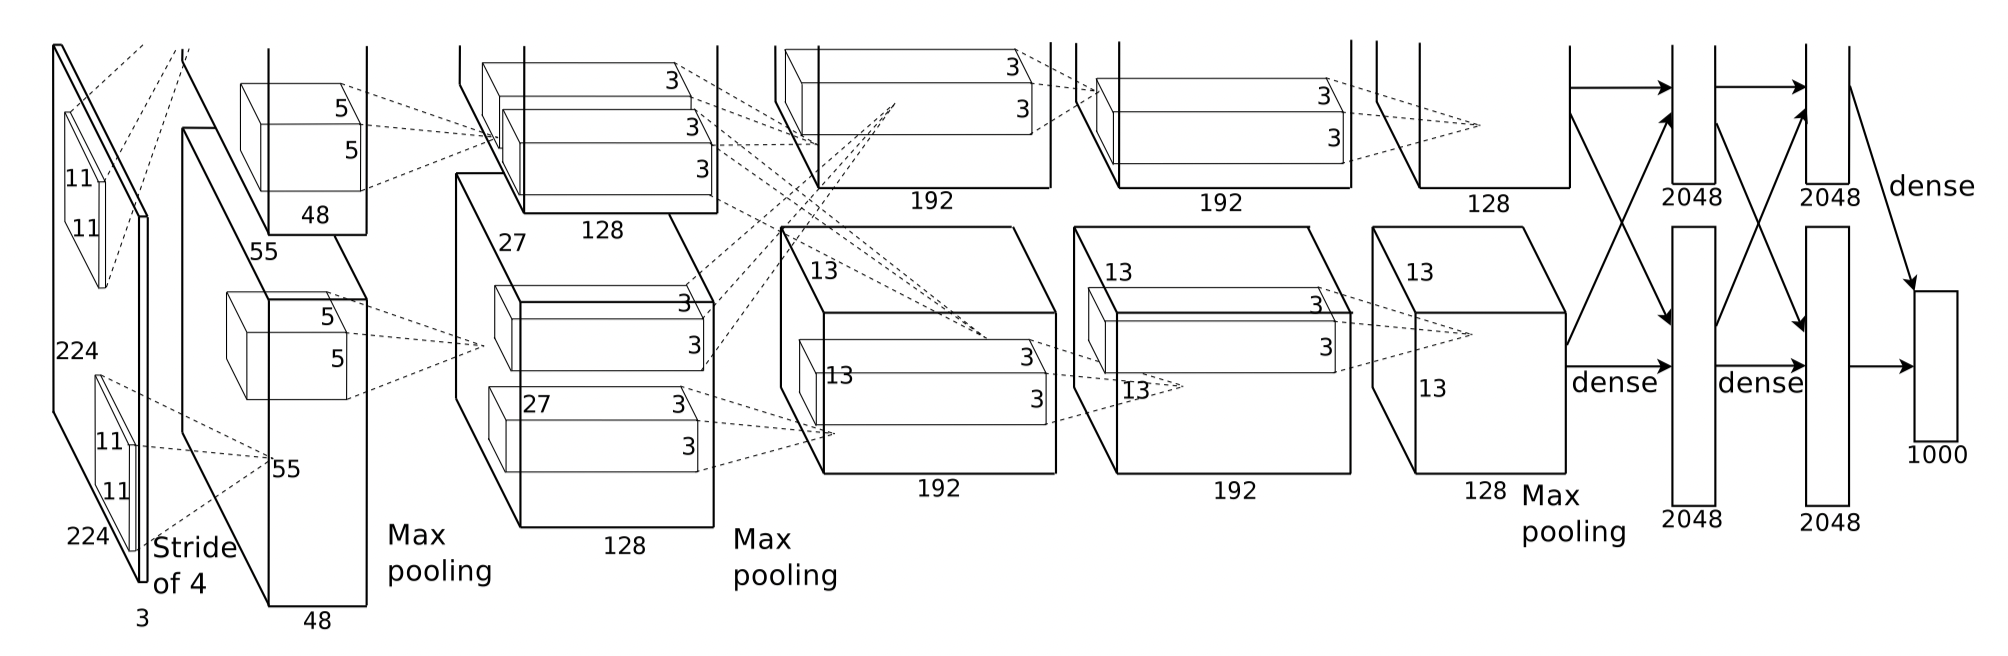
\includegraphics[width=6in]{figures/alex_net.png}
    \caption{AlexNet's Overall Archietecture \cite{AlexNet_2017}} \label{fig:alex_net_architecture}
\end{figure}

Aside from being one of the largest networks and using a parallelization scheme, AlexNet was also one of the first neural networks utilizing ReLUs. At the time, the ReLUs activation function was used instead of the more popular $Tanh$ and $Sigmoid$ functions because AlexNet was designed to focus on improving learning time. Using ReLUs, the model has a faster learning rate, which the author believes would immensely improve the performance of large models with a large data set. Additionally, AlexNet introduces local response normalization (LRN) to help ReLUs with generalization. The non-trainable LRN layer is used after the first and second layers of the network. AlexNet also utilizes a max-pooling layer with a size of 3 and a stride of 2 following the first, second, and fifth layers. The author observes that using an overlapping pooling layer -- i.e., size 3 > stride 2 -- generally reduces the amount of overfitting \cite{AlexNet_2017}. 

Lastly, to adress the overfitting problem when train a large network with large data set, AlexNet utilize data augmentation and dropout technique. For data augmentation, AlexNet randomly select images into batches, resize them to the resolution of $224 \times 224$, generate a copy with horizontal reflection image transformation and a copy with modified intensity for the three RGB channel. These transformed images are generated using CPU while the GPU is training on the previous batch, thus the data augmentation technique can be performed with no addional cost to the performance of the model. 

\begin{itemize}
    \item talk about dropout technique
    \item R-CNN model utilize the AlexNet architect implemented on the Caffe framework. R-CNN model pass each generated ROIs as seperated imaged to AlexNet for feature extraction. Since ROIs role is to find each object location in the image, thus AlexNet can assume each ROI only have exactly one object or one feature. AlexNet also require image input of fixed resolution $224 \times 224$, thus R-CNN transform to the required size by warping all pixels in a bounding box of $227 \times 227$.
\end{itemize}





% and . This mean that in ILSVRC-2010 challenge, AlexNet model  or 


% 


% The version of AlexNet being used in the R-CNN model 


% This is possible due to generated ROIs are consider as seperated images by AlexNet, assume to have exactly one object or one feature within each image, . 

\subsection{The Third Module: Classification With Pre-trained SVM}
% \begin{figure}[H]
%     \caption{rcnn 3rd module notes} \centering
%     \includegraphics[width=6in]{asset/to_remove/rcnn-3module.png}
% \end{figure}